\documentclass[12pt,a4paper,oneside]{article}

\usepackage[utf8]{inputenc}
\usepackage[portuguese]{babel}
\usepackage[T1]{fontenc}
\usepackage{amsmath}
\usepackage{amsfonts}
\usepackage{amssymb}
\usepackage{graphicx}

\usepackage{xcolor}
% Definindo novas cores
\definecolor{verde}{rgb}{0.25,0.5,0.35}
\definecolor{jpurple}{rgb}{0.5,0,0.35}
% Configurando layout para mostrar codigos Java
\usepackage{listings}
\definecolor{mygreen}{rgb}{0,0.6,0}
\definecolor{mygray}{rgb}{0.5,0.5,0.5}
\definecolor{mymauve}{rgb}{0.58,0,0.82}

\usepackage{listings}
\lstdefinelanguage{JavaScript}{
	keywords={typeof, new, true, false, catch, function, return, null, catch, switch, var, if, in, while, do, else, case, break},
	keywordstyle=\color{black}\bfseries,
	ndkeywords={class, export, boolean, throw, implements, import, this},
	ndkeywordstyle=\color{darkgray}\bfseries,
	identifierstyle=\color{black},
	sensitive=false,
	comment=[l]{//},
	morecomment=[s]{/*}{*/},
	commentstyle=\color{black}\ttfamily,
	stringstyle=\color{black}\ttfamily,
	morestring=[b]',
	morestring=[b]",
}

\lstset{ %
	backgroundcolor=\color{white},   % choose the background color; you must add \usepackage{color} or \usepackage{xcolor}
	basicstyle=\small,        % the size of the fonts that are used for the code
	breakatwhitespace=false,         % sets if automatic breaks should only happen at whitespace
	breaklines=true,                 % sets automatic line breaking
	captionpos=b,                    % sets the caption-position to bottom
	commentstyle=\color{mygreen},    % comment style
	deletekeywords={...},            % if you want to delete keywords from the given language
	escapeinside={\%*}{*)},          % if you want to add LaTeX within your code
	extendedchars=true,              % lets you use non-ASCII characters; for 8-bits encodings only, does not work with UTF-8
	frame=single,	                   % adds a frame around the code
	keepspaces=true,                 % keeps spaces in text, useful for keeping indentation of code (possibly needs columns=flexible)
	keywordstyle=\color{blue},       % keyword style
	language=HTML,                 % the language of the code
	otherkeywords={*,...},           % if you want to add more keywords to the set
	numbers=left,                    % where to put the line-numbers; possible values are (none, left, right)
	numbersep=5pt,                   % how far the line-numbers are from the code
	numberstyle=\tiny\color{black}, % the style that is used for the line-numbers
	rulecolor=\color{black},         % if not set, the frame-color may be changed on line-breaks within not-black text (e.g. comments (green here))
	showspaces=false,                % show spaces everywhere adding particular underscores; it overrides 'showstringspaces'
	showstringspaces=false,          % underline spaces within strings only
	showtabs=false,                  % show tabs within strings adding particular underscores
	stepnumber=1,                    % the step between two line-numbers. If it's 1, each line will be numbered
	stringstyle=\color{mymauve},     % string literal style
	tabsize=2,	                   % sets default tabsize to 2 spaces
	title=\lstname,                   % show the filename of files included with \lstinputlisting; also try caption instead of title
	moredelim=**[is][\color{purple}]{@}{@},
}


\author{\\Universidade Federal de Goiás (UFG) - Regional Jataí\\Bacharelado em Ciência da Computação \\Física para Ciência da Computação \\Esdras Lins Bispo Jr.}

\title{\sc \huge Prova (Parte 2)}

\date{02 de dezembro de 2019}

\begin{document}

\maketitle

{\bf ORIENTAÇÕES PARA A RESOLUÇÃO}

\footnotesize

\begin{itemize}
	\item A avaliação é individual, sem consulta;
	\item A pontuação máxima desta avaliação é 10,0 (dez) pontos, sendo uma das 05 (cinco) componentes que formarão a média final da disciplina: dois testes, duas provas e exercícios-bônus;
	\item A média final ($MF$) será calculada assim como se segue
	\begin{eqnarray}
		MF & = & MIN(10, S) \nonumber \\
		S & = & (\sum_{i=1}^{4} 0,2.T_i ) + 0,2.P  + EB \nonumber
	\end{eqnarray}
	em que 
	\begin{itemize}
		\item $S$ é o somatório da pontuação de todas as avaliações,
		\item $T_i$ é a pontuação obtida no teste $i$,
		\item $P$ é a pontuação obtida na prova, e
		\item $EB$ é a pontuação total dos exercícios-bônus.
	\end{itemize}
	\item O conteúdo exigido compreende os seguintes pontos apresentados no Plano de Ensino da disciplina: (2) Movimentos, (3) Trabalho e Energia, (4) Colisões, (7) Projeto de Animação, e (8) Outros Tópicos.
\end{itemize}


\begin{center}
	\fbox{\large Nome: \hspace{10cm}}
	\fbox{\large Assinatura: \hspace{9cm}}
\end{center}

\newpage

\normalsize

\begin{enumerate}
	
	\section*{Substitutiva do Teste 03}

\item (5,0 pt) {\bf (Halliday 2.44)} Um tatu assustado pula verticalmente para cima, subindo $0,6$ m nos primeiros $0,2$ s. (Admita $g= 10$ m/s$^2$).
\begin{enumerate}
	\item Qual é a velocidade do animal ao deixar o solo?
	
	\vspace*{0.3cm}
	
	{\color{blue} {\bf Resposta:} \\
		$y - y_0 = v_0t + \frac{1}{2}at^2$ \\
		$0,6 \mbox{ m} = v_0\times 0,2 \mbox{ s} + \frac{1}{2}(-10 \mbox{ m/s}^2)(0,2 \mbox{ s})^2$ \\
		$0,6 \mbox{ m} = (0,2\mbox{ s})\times v_0  + (-5 \mbox{ m/s}^2)(0,04 \mbox{ s}^2)$ \\
		$0,6 \mbox{ m} = (0,2\mbox{ s})\times v_0  -0,2 \mbox{ m}$ \\
		$0,8 \mbox{ m} = (0,2\mbox{ s})\times v_0$\\
		$(0,2\mbox{ s})\times v_0 = 0,8 \mbox{ m}$\\
		\fbox{$v_0 = \dfrac{0,8 \mbox{ m}}{0,2\mbox{ s}} = 4 \mbox{ m/s}$}\\
	}
	\item Qual é a velocidade na altura de $0,6$ m?
	
	\vspace*{0.3cm}
	
	{\color{blue} {\bf Resposta:} \\
		$v = v_0 + a t$\\
		$v = 4 \mbox{ m/s} + (-10 \mbox{ m/s}^2)\times (0,2 \mbox{ s})$\\
		$v = 4 \mbox{ m/s} -2 \mbox{ m/s}$\\
		\fbox{$v = 2 \mbox{ m/s}$}\\
	}
\end{enumerate}	 
	
	\newpage
	
	\item (5,0 pt) Em JavaScript, você irá escrever a função {\tt emCadaPasso} de acordo com o modelo apresentado abaixo. Você deve substituir apenas as linhas 6, 8 e 9, pelos trechos de código 1, 2 e 3, respectivamente. O objetivo é que a bola azul realize um movimento uniforme (MU) até chegar no limite lateral do {\tt canvas} (sem ultrapassá-lo). Então, ela volta na mesma direção, i.e., ela fará outro MU, só que desta vez com a velocidade negativa (e de mesmo módulo). Garanta que os MUs de ida e volta permaneçam indefinidamente.
	
	\begin{lstlisting}[language=JavaScript]
function emCadaPasso() {    
	bola.x += bola.vx; 
	
	if (bola.x > canvas.width - bola.raio){ 
		bola.x = canvas.width - bola.raio; 
		// TRECHO 1
	}
	if(/* TRECHO 2 */){
		// TRECHO 3
		bola.vx = -bola.vx;
	}
	
	bola.desenhar(contexto); 
}\end{lstlisting}

{\color{blue} {\bf Resposta:}}  \\
\begin{lstlisting}[language=JavaScript]
//TRECHO 1
bola.vx = -bola.vx;

//TRECHO 2
bola.x < bola.raio

//TRECHO 3
bola.x = bola.raio;
\end{lstlisting}

	
	\newpage
	
	\section*{Substitutiva do Teste 04}
	
		\item (5,0 pt) {\bf (Halliday PG.4.5)} A Figura 1 mostra três situações nas quais projéteis iguais são lançados do solo (a partir do mesmo nível) com a mesma velocidade escalar e o mesmo ângulo. Entretanto, os projéteis não caem no mesmo terreno. Ordene as situações de acordo com a velocidade escalar final dos projéteis imediatamente antes de aterrissarem, começando pela maior. {\bf Justifique a sua resposta.}
	
	\begin{figure}[htb]
		\begin{center}
			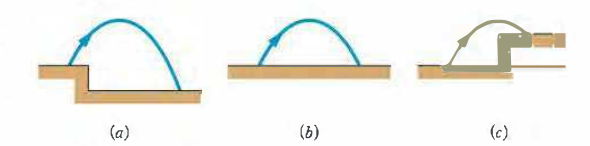
\includegraphics[scale=0.8]{images/fig1}
		\end{center}
		\caption{Lançamento de projéteis em três situações diferentes.}
	\end{figure}

	{\color{blue} {\bf Resposta:} Após atingir a altura máxima, depois do lançamento, os projéteis levam tempo diferentes até a colisão com o solo. Devido às diferenças de níveis no terreno, o tempo na situação (a) é maior que na situação (b); e o tempo na situação (b) é maior do que na situação (c). Logo, $t_a >  t_b > t_c$. Como a velocidade escalar do projétil será maior se houver um tempo maior de queda, logo $|v_a| > |v_b| > |v_c|$.
	}
	
	\newpage 
	
	\item (5,0 pt) Em JavaScript, você irá escrever a função {\tt emCadaPasso} de acordo com o modelo apresentado abaixo. Você deve substituir apenas as linhas 8, 11 e 15, pelos trechos de código 1, 2 e 3, respectivamente. O objetivo é que a bola azul realize um movimento oblíquo de forma que haja uma coeficiente de restituição de 60\% ao colidir com as paredes laterais ou de 90\% com o solo, simulando o comportamento de uma bola colidindo nas paredes de uma sala. O movimento da bola permanecerá indefinidamente, respeitando as condições já mencionadas.
	
	\begin{lstlisting}[language=JavaScript]
function emCadaPasso() {    
	bola.x += bola.vx;
	bola.vy += bola.ay;
	bola.y += bola.vy;
	
	if (bola.y > canvas.height - bola.raio){ 
		bola.y = canvas.height - bola.raio; 
		// TRECHO 1
	}
	if(bola.x < bola.raio){
		// TRECHO 2
		bola.vx = -bola.vx*0.6;
	}
	if(bola.x > canvas.width - bola.raio){
		// TRECHO 3 
	}
	
	bola.desenhar(contexto); 
}\end{lstlisting}

{\color{blue} {\bf Resposta:}}  \\
\begin{lstlisting}[language=JavaScript]
//TRECHO 1
bola.vy = -bola.vy*0.9;

//TRECHO 2
bola.x = bola.raio;

//TRECHO 3
bola.x = canvas.width - bola.raio;
bola.vx = -bola.vx*0.6;
\end{lstlisting}
	
	\end{enumerate}

\newpage

\section{Fórmulas Auxiliares}

\subsection{Movimento Uniforme (MU)}

\begin{enumerate}
	\item $x = x_0 + vt$ 
\end{enumerate}

\subsection{Movimento Uniformemente Variado (MUV)}

\begin{enumerate}
	\item $x - x_0 = v_0t + \frac{1}{2}at^2$ 
	\item $v = v_0 + at$ 
	\item $x - x_0 = \frac{1}{2}(v_0 + v)t$ 
	\item $x - x_0 = vt - \frac{1}{2} a t^2$
	\item $v^2 = v_0^2 + 2a(x - x_0)$
\end{enumerate}

\section*{js/principal.js}

\begin{lstlisting} [language=JavaScript]
var canvas = document.getElementById('canvas');
var contexto = canvas.getContext('2d');

var bola = new Bola(50, '#0000ff');
inicializar("emCadaPasso");

window.onload = init;

function init() {
	setInterval(emCadaPasso, 1000/60);
};
\end{lstlisting}

\newpage

\section*{js/Bola.js}

\begin{lstlisting}[language=JavaScript]
function Bola(raio, cor) {
	this.raio = raio;
	this.cor = cor;
	this.x = 0;
	this.y = 0;
	this.vx = 0;
	this.vy = 0;
}

Bola.prototype.desenhar = function (contexto) {
	contexto.clearRect(0, 0, canvas.width, canvas.height);
	contexto.fillStyle = this.cor;
	contexto.beginPath();
	contexto.arc(this.x, this.y, this.raio, 0, 2 * Math.PI, true);
	contexto.closePath();
	contexto.fill();
};
\end{lstlisting}

\section*{js/inicializacao.js}

\begin{lstlisting}[language=JavaScript]
function bolabaseEsquerda(margem) {
	bola.x = bola.raio + margem;
	bola.y = canvas.height - bola.raio - margem;
}

function inicializar(valor){
	switch(valor){
		case "emCadaPasso":
			bolaBaseEsquerda(30);
			bola.vy = -120/60; 
			bola.vx = 60/60;
			bola.ay = 98/60;
			break;
	}
}
\end{lstlisting}

\end{document}